\chapter{Lógica proposicional}
\pagenumbering{arabic}
\setcounter{page}{1}
$\\$
\section{Introducción}
Antes de comenzar con definiciones rigurosas, conviene dar una breve explicación sobre la motivación de la lógica proposicional, a la que dedicaremos este capítulo. Un aspecto común de los lenguajes naturales (como el español o el chino) es la ambigüedad de ciertas expresiones, lo cual dificulta las intenciones usuales de la ciencia, a saber, la precisión en la comunicación y la distinción clara de aquello que se comunica. De aquí nace una necesidad evidente, que es cubierta por los lenguajes artificiales y, entre ellos, la lógica formal. \

Debemos aclarar entonces cuál es nuestro objeto de estudio. Fijémonos en lo siguiente: existen ciertos elementos del lenguaje que no cambian si los traducimos a otro idioma, por ejemplo. Nos referimos a lo que se denomina como \textit{conectivas lógicas}, es decir, `no' (negación), `o' (disyunción), `y' (conjunción), `si... entonces' (implicación material) y `si y solo si' (equivalencia). Obviamente, podemos usar múltiples expresiones distintas para referirnos a cada una de ellas, pero su función en el lenguaje natural no cambia. Por esto mismo podemos formalizarlas y estudiarlas desde el punto de vista matemático.  

Ahora bien, a fin de sistematizar nuestro lenguaje, introducimos una serie de símbolos que se referirán a las entidades correspondientes del lenguaje natural. Conviene puntualizar de nuevo que estas traducciones, es decir, estas `asignaciones de significados' \textit{no} son únicas. Esto lo veremos más adelante. Entonces tenemos: $\neg$ (negación), $\lor$ (disyunción), $\land$ (conjunción), $\rightarrow$ (implicación material) y $\leftrightarrow$ (equivalencia). \

Los otros elementos básicos que constituirán nuestro lenguaje formal son las \textit{proposiciones}. Con el fin de no entrar en cuestiones semánticas que exceden nuestro estudio, establecemos la siguiente:

\begin{definition}\label{def: prop}
    Una proposición es un enunciado que puede ser verdadero o falso. 
\end{definition}
Como con las conectivas, introducimos una serie de \textit{símbolos de proposición} para referirnos formalmente a las proposiciones. Denotamos por $SP$ al conjunto de todos estos símbolos.

Así, el enunciado `Todos los solteros son hombres no casados' es una proposición, mientras que `¿Va a llover mañana?' no lo es. Por otro lado, `César conquistó las Galias y combatió contra Vercingétorix' admite una descomposición como conjunción de dos proposiciones. Evidentemente, esta reducción a proposiciones más simples tiene que parar eventualmente; así llegamos a lo que denominamos \textit{proposiciones atómicas}. Esto nos permitirá, una vez determinada la verdad o falsedad de estas proposiciones atómicas, hallar la de todas las proposiciones que se compongan de ellas mediante la aplicación de las conectivas lógicas (antiguamente llamadas \textit{proposiciones moleculares}). \

Las proposiciones atómicas se representan entonces por los elementos de $SP$. Añadimos, por motivos que serán aclarados más adelante, dos elementos $\top$ y $\bot$, que se refieren a la \textit{proposición idénticamente verdadera} y a la \textit{proposición idénticamente falsa}, respectivamente\footnote{En realidad, como veremos, al igual que $\neg,\land,\lor,\to$ y $\leftrightarrow$ son conectivas binarias, $\top$ y $\bot$ pueden considerarse conectivas 0-arias.}. Es decir, 

\begin{definition}\label{def : at}

     Definimos el conjunto de las proposiciones atómicas como:
    \[
        AT := SP\cup \{\top, \bot\}
    \]
\end{definition}


\begin{definition}(Alfabeto)
    Dado un conjunto de símbolos de proposiciones $SP$, se denomina alfabeto a:
    \[
        A_{SP} = SP\cup\{\neg, \land, \lor, \rightarrow, \leftrightarrow, (, ),\top, \bot\},
    \]
    obtenido añadiendo a $SP$ los símbolos $\top$ y $\bot$, las conectivas lógicas $\neg, \land, \lor, \rightarrow, \leftrightarrow$, y los paréntesis, $(,)$.
\end{definition}    


\begin{definition}(Cierre de Kleene)
    Dado un conjunto de símbolos $A$, definimos el cierre de Kleene de $A$, $A^*$, como el conjunto de las concatenaciones de elementos de $A$ junto con $\epsilon$, el \textit{espacio vacío} o en blanco.
\end{definition}

\begin{example} Dado $A = \{a, b\}$, le corresponde 
\[
    A^* = \{\epsilon, a, b, ab, ba, aab, baa, aba, ...\}
\]
\end{example}
\begin{example}
    $A_{SP}^*$ será el conjunto de todas las concatenaciones de elementos de $A_{SP}$, junto con $\epsilon$.
\end{example}

Una vez que disponemos de los elementos básicos de la sintaxis del lenguaje y sus sucesivas combinaciones, nos interesa definir las expresiones que están `bien formadas', es decir, queremos excluir de nuestro lenguaje  concatenaciones de símbolos como `$)) \leftrightarrow \varphi$'.

\begin{definition}\label{def:PROP_{SP}}(Proposiciones posibles)
Se define el conjunto de proposiciones posibles,  $PROP_{SP}$, como la intersección de todos los subconjuntos de $A_{SP}^*$ que verifican:
\begin{enumerate}
    \item $SP \subseteq PROP_{SP}$.
    \item Si $\phi\in PROP_{SP}$, entonces $(\neg \phi) \in PROP_{SP} $.
    \item Si $\phi_1, \phi_2 \in PROP_{SP}$ y $\square\in \{\land, \lor, \rightarrow, \leftrightarrow\}$, entonces $(\phi_1 \square\  \phi_2) \in PROP_{SP}$.
\end{enumerate}
\end{definition}
Es fácil comprobar que $PROP_{SP}$ también cumple estas tres propiedades, por tanto decimos que es el mínimo subconjunto que las verifica. También podemos obtener $PROP_{SP}$ de forma constructiva:

\begin{prop} Se define $P_0 := SP$ y para cada $n\in\N$:
\[
    P_n := P_{n-1} \cup \{(\neg \phi): \phi\in P_{n-1}\}\cup \{ (\phi_1 \square\  \phi_2): \phi_1, \phi_2\in P_{n-1},  \square\in \{\land, \lor, \rightarrow, \leftrightarrow\}\}.
\]
Entonces $P := \bigcup_{n=0}^\infty P_n$ coincide con $PROP_{SP}$.
\begin{proof} 
Comenzamos comprobando $P\subseteq PROP_{SP}$. Para ello, comprobamos por inducción que $P_n\subseteq PROP_{SP}$ $\forall n \in \mathbb{N}$. \\ \\
Está claro que $P_0\subseteq PROP_{SP}$, ya que $PROP_{SP}$ cumple la propiedad 1.
Ahora, suponiendo que $P_n\subseteq PROP_{SP}$, por las propiedades 2 y 3, $\{(\neg \phi): \phi\in P_{n-1}\}\cup \{ (\phi_1 \square\  \phi_2): \phi_1, \phi_2\in P_{n-1},  \square\in \{\land, \lor, \rightarrow, \leftrightarrow\}\}$ también estarán  contenidos en $PROP_{SP}$. Por tanto, $P_{n+1}\subseteq PROP_{SP}$, y hemos acabado la inducción. \\ \\
Veamos ahora que $PROP_{SP}\subseteq P$. Para ello nos basta comprobar que $P$ cumple las tres propiedades de la definición ~\ref{def:PROP_{SP}}. La propiedad $1$ es directa, pasamos a comprobar las propiedades 2 y 3. \\ \\
Dado $\varphi \in P$, existe $n\in \N\cup\{0\}$ tal que $\varphi \in P_n$ luego $(\neg \varphi) \in P_{n+1}$ por lo que $(\neg\varphi) \in P$. \\ \\
Sean $\varphi_1, \varphi_2 \in P$ y sea $\square\in \{\land, \lor, \rightarrow, \leftrightarrow\}$. Tomamos $n\in\N$ tal que $\varphi_1, \varphi_2 \in P_n$ (para cada uno existe al menos un natural: basta tomar el mayor). Luego $(\phi_1 \square\  \phi_2)\in P_{n+1}$ y por lo tanto también pertenece a $P$. \\ \\
\end{proof}
\end{prop}
A partir de ahora, usaremos para mayor brevedad el símbolo $\square$ como intercambiable por $\land, \lor, \rightarrow$ o $\leftrightarrow$ a no ser que se indique lo contrario. $\\$


Básicamente, el resultado anterior nos dice que podemos construir cualquier proposición partiendo de proposiciones atómicas y creando proposiciones más complicadas a partir de ellas usando las conectivas. Esta forma de verlo da lugar al siguiente concepto:

\begin{definition}(Secuencia de formación)
Definimos una \textit{secuencia de formación} para cierto $\varphi\in A_{SP}^*$ como una sucesión finita $\langle\varphi_1,\dots,\varphi_n\rangle$ de elementos de $A_{SP}^*$ tal que $\varphi_n=\varphi$ y para cada $i\leq n$, se da alguna de estas tres opciones:
\begin{itemize}
    \item $\varphi_i\in AT$.
    \item $\varphi_i=(\neg \varphi_j)$, para cierto $j<i$.
    \item $\varphi_i=(\varphi_j\square\varphi_k)$, para ciertos $j,k<i$.
\end{itemize}
\end{definition}

Como veremos en los ejercicios, toda proposición puede construirse mediante una secuencia de formación, y recíprocamente si $\varphi$ tiene una secuencia de formación, entonces $\varphi\in PROP_{SP}$.

\section{Inducción estructural y recursión}

Análogamente al método de inducción en los naturales, el método de inducción estructural nos servirá para demostrar que todas las fórmulas cumplen una \textit{propiedad}\footnote{No hemos definido rigurosamente el concepto de "propiedad", pero esencialmente significa algo que las proposiciones pueden cumplir o no. Una forma rigurosa de definir propiedad consiste en definirla como un subconjunto $P\subseteq PROP_{SP}$, de modo que decimos que una proposición cumple la propiedad $P$ si y solo si pertenece a $P$.} en dos pasos: demostrar que todas las proposiciones atómicas cumplen dicha propiedad, y demostrar que si dos proposiciones $\varphi_1,\varphi_2$ cumplen una propiedad, entonces $(\neg\varphi_1)$ y $(\varphi_1\square\varphi_2)$ también la cumplen.$\\$

\begin{prop} (Inducción estructural) Supongamos que queremos probar $P(\varphi)$\footnote{Usamos la notación $P(\varphi)$ para decir que la fórmula $\varphi$ cumple la propiedad $p$.} para todo $\varphi\in PROP_{SP}$ (siendo $P$ una propiedad cualquiera). Entonces basta comprobar que:
\begin{enumerate}
    \item $P(\varphi)$ para toda $\varphi\in AT$.
    \item Si $P(\varphi)$ entonces $P((\neg \varphi))$.
    \item Si $P(\varphi_1)$ y $P(\varphi_2)$ entonces $P((\varphi_1 \square \varphi_2))$.
\end{enumerate}
\begin{proof}
Si una propiedad $P$ cumple 1, 2 y 3, entonces el conjunto de proposiciones que cumplen $P$ cumple las tres propiedades de \ref{def:PROP_{SP}}, por tanto contiene a $PROP_{SP}$. \\
\end{proof}
\end{prop}

\begin{example} Definamos $P(\varphi)$ como la propiedad de $|\varphi|_) = |\varphi|_($, siendo $|\varphi|_)$ el número de símbolos $)$ en la fórmula $\varphi$ y $|\varphi|_($ el número de $($\footnote{En general, siendo $*$ un símbolo, podemos denotar $|\varphi|_*$ al número de símbolos $*$ en la fórmula $\varphi$.}. Vamos a comprobar por inducción estructural que todas las proposiciones cumplen esta propiedad:
\begin{enumerate}
    \item Para cualquier $\varphi\in AT$ se verifica trivialmente $|\varphi|_) = |\varphi|_( = 0$, luego $P(\varphi)$.
    \item Supongamos $P(\varphi)$ con $\varphi\in PROP_{SP}$, entonces $|\varphi|_( = |\varphi|_)$ y por tanto:
    \[
        |(\neg\varphi)|_( = |\varphi|_(+1 = |\varphi|_)+1 = |(\neg\varphi)|_)
    \]
    luego $P((\neg\varphi))$.
    \item Supongamos $P(\varphi),P(\psi)$ con $\varphi,\psi\in PROP_{SP}$, entonces:
    \[
        |(\varphi\square\psi)|_(=|\varphi|_(+|\psi|_(+1=|\varphi|_)+|\psi|_)+1=|(\varphi\square\psi)|_)
    \]
    luego $P((\varphi\square\psi))$.
\end{enumerate}
\end{example}

\begin{definition} (Prefijos) Sea $A$ un alfabeto y sea $w\in A^*$. Decimos que $w'$ es prefijo de $w$ si existe $w''$ tal que $w = w' w''$, es decir, si $w = w_1 w_2 ... w_n$ entonces existe $0\leq k\leq n$ tal que $w' = w_1 ... w_k$.$\\$
Decimos además que un prefijo $w'$ es prefijo propio de $w$ si es distinto de $w$ y $\epsilon$.
\end{definition}

\begin{example} Sea $A := \{a, b\}$ y sea $w := aababb$. Entonces sus prefijos son $\epsilon,a,aa,aab,aaba,aabab,aababb$, correspondientes a $k=0,1,2,3,4,5,6$, respectivamente, y sus prefijos propios son $a,aa,aab,aaba,aabab$.
\end{example}

\begin{prop} Si $\varphi'$ es prefijo propio de $\varphi$, entonces $|\varphi'|_) < |\varphi'|_($.
\begin{proof} Se demuestra por inducción estructural.
\begin{enumerate}
    \item Si $\varphi\in AT$ no tiene prefijos propios luego se cumple la afirmación.
    \item Sea $\varphi\in PROP_{SP}$ cumpliendo la propiedad del enunciado y sea $\varphi'$ un prefijo propio de $(\neg \varphi)$. Existen cuatro casos:
    \begin{enumerate}
        \item $\varphi' = ($, entonces $|\varphi'|_( = 1 > 0 = |\varphi'|_)$-
        \item $\varphi' = (\neg$, ocurre lo mismo que antes.
        \item $\varphi' = (\neg \varphi''$ con $\varphi''$ prefijo propio de $\varphi$ entonces por inducción se verifica $|\varphi''|_) < |\varphi''|_($. Ahora bien, $|\varphi'|_( = |\varphi''|_(+1$  y $|\varphi'|_) = |\varphi''|_)$ luego:
        \[
            |\varphi'|_) < |\varphi'|_(
        \]
        \item $\varphi' = (\neg \varphi$, que es directo. 
    \end{enumerate}
    \item Se hace de forma similar al apartado anterior. Basta probar con los prefijos $(,\ (\varphi_1',\ (\varphi_1,\ (\varphi_1\square,\ (\varphi_1\square\varphi_2'$ y $(\varphi_1\square\varphi_2$.
\end{enumerate}
    
\end{proof}
\end{prop}

 En próximas secciones será útil, dado un conjunto $A$, definir una función $H: PROP_{SP} \rightarrow A$ conociendo su restricción a $AT$, y suponiendo que podemos calcular $H((\neg \varphi))$ y $H((\varphi\square\psi))$ en función de $H(\varphi)$ y $H(\psi)$.
 Si la función $H$ queda bien definida así, diremos que está \textit{definida de forma recursiva}. La siguiente proposición nos garantiza que podemos definir funciones de esta forma:
 
 \begin{prop} El esquema de definición recursiva da como resultado una única función, es decir, dadas:
\begin{enumerate}
    \item $H_{AT}: AT \rightarrow A$.
    \item $H_{\neg}: A \rightarrow A$.
    \item $H_{\square}: A \times A \rightarrow A$.
\end{enumerate}
existe una única función $H: PROP_{SP} \rightarrow A$ tal que:
\begin{enumerate}
    \item $H(\varphi) = H_{AT}(\varphi)$, para toda $\varphi \in AT$.
    \item $H((\neg \varphi)) = H_{\neg}(H(\varphi))$.
    \item $H((\varphi_1 \square \varphi_2)) = H_{\square}(H(\varphi_1), H(\varphi_2))$, para cada $\square\in \{\land, \lor, \rightarrow, \leftrightarrow\}$.
\end{enumerate}
\begin{proof}
     Se omite la demostración.
\end{proof}
\end{prop}

\begin{example} Sea $H: PROP_{SP} \rightarrow \mathbb{N}$ la función $|.|_($ definida anteriormente. Podemos definirla de manera recursiva:
\begin{enumerate}
    \item $H(\varphi) = 0$, para toda $\varphi \in AT$.
    \item $H((\neg \varphi)) = H(\varphi) + 1$.
    \item $H((\varphi_1 \square \varphi_2)) = H(\varphi_1) + H(\varphi_2) + 1$.
\end{enumerate}
Nótese como en ocasiones omitimos las funciones auxiliares y usamos la notación $H$ para referirnos a $H$, $H_{AT}$, $H_{\neg}$ y $H_{\square}$. Este abuso de notación no suele dar lugar a confusión.
\end{example}



\begin{example} Podemos definir recursivamente una función que nos lleve cada fórmula al conjunto de todas sus subfórmulas, es decir,  $\text{\textit{\text{\textit{SUB}}}}: PROP_{SP} \rightarrow \mathcal{P} (PROP_{SP})$\footnote{Dado un conjunto X, denotamos por $\mathcal{P}(X)$ a su potencia, es decir, el conjunto de subconjuntos de X.} tal que:
\begin{enumerate}
    \item $\text{\textit{SUB}}(\varphi) = \{\varphi\}$, para toda $\varphi \in AT$.
    \item $\text{\textit{SUB}}((\neg \varphi)) = \text{\textit{SUB}}(\varphi) \cup \{(\neg \varphi)\}$.
    \item $\text{\textit{SUB}}((\varphi_1 \square \varphi_2)) = \text{\textit{SUB}}(\varphi_1) \cup \text{\textit{SUB}}(\varphi_2) \cup \{(\varphi_1 \square \varphi_2)\}$.
\end{enumerate}
\end{example} 

\section{Eliminación de paréntesis}
Para conseguir una notación más compacta, podemos establecer una notación que use menos paréntesis cuando nos convenga. Sin embargo, la omisión de paréntesis puede dar lugar a ambigüedades en las fórmulas, por ejemplo,
\[p\to q \to r\]
podría simbolizar dos fórmulas distintas:
\begin{itemize}
    \item $((p\to q)\to r)$
    \item $(p\to (q\to r))$
\end{itemize}
Para evitar este tipo de situaciones, necesitamos las siguientes reglas de omisión de paréntesis:
\begin{enumerate}
    \item Los paréntesis externos pueden omitirse. Esto no da lugar a ambigüedad.
    \item Las conectivas se aplicarán en este orden: $\neg, \land, \lor, \to, \leftrightarrow$.
    \item Cuando hay varias conectivas del mismo tipo seguidas, se asocia siempre por la izquierda.
\end{enumerate}
Algunos ejemplos de aplicación de estas reglas:$\\[8pt]$
\begin{equation*}
\begin{array}{ccc}
     \neg p\lor p  & \text{es} & ((\neg p)\lor p)\\
     \neg p\land q\lor s\to t\leftrightarrow r & \text{es} & 
     (((((\neg p)\land q)\lor s)\to t)\leftrightarrow r)\\
     p\to q\to s & \text{es} & ((p\to q)\to s)\\
     p\land q\leftrightarrow\neg s\to t\lor r & \text{es} & ((p\land q)\leftrightarrow((\neg s)\to (t\lor r))) \\
     t\leftrightarrow p\to \neg q\lor p\to s & \text{es} & 
     (t \leftrightarrow((p\to ((\neg q)\lor p))\to s))
\end{array}
\end{equation*}

Comprobaremos que las conectivas $\land$ y $\lor$ son asociativas y conmutativas, por tanto, en ese sentido, no importa el orden en que se asocien. De modo que, cuando una conectiva se repita varias veces seguidas, podemos usar la siguiente notación:
\[\bigwedge\limits_{i\in I} p_i:=p_{i_1}\land\dots\land p_{i_n}\]
\[\bigvee\limits_{i\in I} p_i:=p_{i_1}\lor\dots\lor p_{i_n},\]
siendo $I=\{i_1,\dots,i_n\}$ un conjunto finito de índices.$\\$
Establecemos además el siguiente convenio,

\[\bigwedge\limits_{i\in \emptyset} p_i:=\top\]
\[\bigvee\limits_{i\in \emptyset} p_i:=\bot,\]
que será consistente con el comportamiento semántico de $\lor$ y $\land$.



\section{Asignaciones de verdad}

Hasta ahora hemos venido considerando cuestiones sintácticas sobre las fórmulas. Lo que queremos ahora es abordar su semántica, esto es, su comportamiento cuando les damos una interpretación determinada. Nos interesa, por tanto, estudiar qué significa que una proposición se siga de otra independientemente de la traducción que hagamos al lenguaje natural, esto es, la noción de \textit{consecuencia lógica}. Así, por ejemplo, queremos que $q$ se siga de $p \land (p \rightarrow q)$ independientemente de cómo se traduzcan $p$ y $q$ informalmente. Es decir, exigimos que, sea cual sea la traducción de $p \land (p \rightarrow q)$, si es verdadera entonces la de $q$ tiene que serlo también.  Siguiendo la definición ~\ref{def: prop}, 

\begin{definition}
Definimos el conjunto de valores de verdad, $Bool = \{V, F\}$, donde $V$ es \textit{la verdad} y $F$ es \textit{la falsedad}\footnote{Nada nos impide considerar casos en que $Bool$ sea infinito numerable, o incluso no numerable, pero la lógica concebida clásicamente es bivalente, esto es, solo consta de dos valores de verdad.}.
\end{definition}

Una vez que disponemos de $Bool$ podemos definir la aplicación que nos lleva cada proposición a su valor de verdad correspondiente. Vamos a definir esta aplicación de forma recursiva, es decir, primero lo haremos para las fórmulas atómicas y después describiremos reglas para deducirla en el resto de fórmulas.

\begin{definition}(Valoración) Sea el conjunto $Bool = \{V, F\}$. Una valoración o evaluación es una función $v: SP \rightarrow Bool$. 
\end{definition}
Un alfabeto de $n$ letras tiene $2^n$ valoraciones distintas.$\\$

Para definir la valoración de proposiciones, vamos a necesitar una forma de interpretar las conectivas. Con este fin, a cada conectiva le asociaremos una aplicación, que definiremos caso a caso en formato de tabla de verdad:

\begin{enumerate}
\item $v_{\neg}: Bool \rightarrow Bool$;
\begin{table}[H]
\begin{center}
\begin{tabular}{|c|c|}
\hline
$\varphi$ & $v_{\neg}(\varphi)$ \\
\hline \hline
V & F \\ \hline
F & V \\ \hline
\end{tabular}
\end{center}
\end{table}
\item $v_\land, v_\lor, v_\rightarrow, v_\leftrightarrow: Bool \times Bool \rightarrow Bool$;
\begin{table}[H]
\begin{center}
\begin{tabular}{|c|c|c|c|c|c|}
\hline
$\varphi_1$ & $\varphi_2$ & $v_{\land}(\varphi_1, \varphi_2)$ & $v_{\lor}(\varphi_1, \varphi_2)$ & $v_{\rightarrow}(\varphi_1, \varphi_2)$ & $v_{\leftrightarrow}(\varphi_1, \varphi_2)$ \\
\hline \hline
V & V & V & V & V & V\\ \hline
V & F & F & V & F & F\\ \hline
F & V & F & V & V & F\\ \hline
F & F & F & F & V & V\\ \hline
\end{tabular}
\end{center}
\end{table}
\end{enumerate}
Decimos que la conectiva binaria $\land$ es un operador conmutativo ya que $v_\land(V,F)=v_\land(F,V)$. $\lor$ y $\leftrightarrow$ también son conmutativas.
\begin{definition}\label{def : ext}(Extensión) Dada la valoración $v: SP \rightarrow Bool$, definimos recursivamente su \textit{extensión}, $\hat{v}: PROP_{SP} \rightarrow Bool$:
\begin{enumerate}
    \item $\hat{v}(\bot) = F$.
    \item $\hat{v}(\top) = V$.\footnote{Aquí es donde hemos dado sentido a la definición que dimos de $\top$ y $\bot$ en ~\ref{def : at}.}
    \item $\hat{v}(\varphi) = v(\varphi)$, para toda $\varphi \in SP$.
    \item $\hat{v}((\neg \varphi)) = v_{\neg}(\hat{v}(\varphi))$.
    \item $\hat{v}((\varphi_1 \square \varphi_2)) = v_{\square}(\hat{v}(\varphi_1), \hat{v}(\varphi_2))$.
\end{enumerate}
\end{definition}


\begin{comment}

\begin{definition}\label{def : ext}(Extensión) Se definen las siguientes aplicaciones:
\begin{enumerate}
    \item $v_{\neg}: Bool \rightarrow Bool$
    \item $v_\land, v_\lor, v_\rightarrow, v_\leftrightarrow: Bool \times Bool \rightarrow Bool$.
\end{enumerate}
Definimos estas funciones caso a caso en formato de tabla de verdad:
\begin{table}[H]
\begin{center}
\begin{tabular}{|c|c|}
\hline
$\varphi$ & $v_{\neg}(\varphi)$ \\
\hline \hline
V & F \\ \hline
F & V \\ \hline
\end{tabular}
\end{center}
\end{table}


\begin{table}[H]
\begin{center}
\begin{tabular}{|c|c|c|c|c|c|}
\hline
$\varphi_1$ & $\varphi_2$ & $v_{\land}(\varphi_1, \varphi_2)$ & $v_{\lor}(\varphi_1, \varphi_2)$ & $v_{\rightarrow}(\varphi_1, \varphi_2)$ & $v_{\leftrightarrow}(\varphi_1, \varphi_2)$ \\
\hline \hline
V & V & V & V & V & V\\ \hline
V & F & F & V & F & F\\ \hline
F & V & F & V & V & F\\ \hline
F & F & F & F & V & V\\ \hline
\end{tabular}
\end{center}
\end{table}

Dada la valoración $v: SP \rightarrow Bool$, definimos recursivamente su \textit{extensión}, $\hat{v}: PROP_{SP} \rightarrow Bool$:
\begin{enumerate}
    \item $\hat{v}(\bot) = F$.
    \item $\hat{v}(\top) = V$.\footnote{Aquí es donde hemos dado sentido a la definición que dimos de $\top$ y $\bot$ en ~\ref{def : at}.}
    \item $\hat{v}(\varphi) = v(\varphi)$, para toda $\varphi \in SP$.
    \item $\hat{v}((\neg \varphi)) = v_{\neg}(\hat{v}(\varphi))$.
    \item $\hat{v}((\varphi_1 \square \varphi_2)) = v_{\square}(\hat{v}(\varphi_1), \hat{v}(\varphi_2))$.
\end{enumerate}
\end{definition}


\end{comment}
La propia definición nos da un método para calcular los valores de verdad de fórmulas en función de los de sus símbolos:

\begin{example}
Encontremos el valor de verdad de $p\land \neg q \to r \lor s$, siendo $v$ una valoración que cumple $v(p)=v(q)=V,v(r)=v(s)=F$:
\begin{enumerate}
    \item $\hat{v}(\neg q)=v_\neg(\hat{v}(q))=v_\neg(V)=F$.
    \item $\hat{v}(p\land \neg q)=v_\land(\hat{v}(p),\hat{v}(\neg q))=v_\land(V,F)=F$.
    \item $\hat{v}(r\lor s)=v_\lor(\hat{v}(r),\hat{v}(s))=v_\lor(F,F)=F$.
    \item Finalmente, $\hat{v}(p\land \neg q \to r\lor s)=v_\to(\hat{v}(p\land \neg q),\hat{v}(r\lor s))=v_\to(F,F)=V$.
\end{enumerate}

\end{example}



\begin{definition}(satisfactibilidad) Dada $v: SP \rightarrow Bool$ y $\varphi \in PROP_{SP}$ se dice que $v$ satisface $\varphi$, y se escribe como $v \vDash \varphi$, si y solo si $\hat{v}(\varphi) = V$. Si $\hat{v}(\varphi) = F$, escribimos $v \nvDash \varphi$.
\end{definition}$\\$
En virtud de la definición anterior, podemos clasificar cada fórmula $\varphi$ como:
\begin{itemize}
    \item \textit{satisfactible}, si existe alguna valoración $v$ tal que $v \vDash \varphi$. 
    \begin{itemize}
        \item \textit{Tautología}, si $v \vDash \varphi$ para toda valoración $v$.
        \item \textit{Contingencia}, si es satisfactible pero no tautología.
    \end{itemize}
    \item \textit{Contradicción}, si no es satisfactible. 
\end{itemize}


\begin{example} La fórmula $p \land q \rightarrow r \leftrightarrow (p \rightarrow q) \rightarrow r$ es contingencia. Invitamos al lector a que realice la tabla de verdad correspondiente.
\end{example}

\begin{definition}(Conjunto de modelos) Dado $\Phi \subseteq PROP_{SP}$, el conjunto de modelos de $\Phi$ se define como:
$$Mod(\Phi) := \{v: SP \rightarrow Bool \ | \ \forall \varphi \in \Phi \ v \vDash \varphi \}$$
\end{definition}

\begin{definition}(Satisfactibilidad) Sea $\Phi \subseteq PROP_{SP}$.$\\[5pt]$
$\Phi$ se dice satisfactible, y se escribe $Sat(\Phi)$, si $Mod(\Phi) \neq \emptyset$.$\\[5pt]$
$\Phi$ se dice insatisfactible, y se escribe $Insat(\Phi)$, si $Mod(\Phi) = \emptyset$. $\\$
\end{definition}

Ahora llegamos a la definición del concepto que ha motivado nuestro estudio inicial de la semántica.

\begin{definition}(Consecuencia lógica) Sea $\varphi \in PROP_{SP}$. Decimos que $\varphi$ es consecuencia lógica de $\Phi$, $\Phi \vDash \varphi$, si y solo si $Mod(\Phi) \subseteq Mod(\{\varphi\})$. \\ \\
Esto equivale a decir que toda asignación de verdad que satisface todos los elementos de $\Phi$ también satisface $\varphi$.\\ \\
\noindent De ahora en adelante, escribimos $Mod(\varphi)$ en vez de $Mod(\{\varphi\})$.
\end{definition}

\begin{example} Dado $\Phi$ tal que $Insat(\Phi)$, se sigue de la anterior definición que $\Phi \vDash \varphi$, para cualquier $\varphi$.
\end{example}
A continuación presentamos algunos resultados básicos de semántica.

\begin{prop} \mbox{}
\begin{enumerate}
    \item $Mod(\emptyset) = \{v | v: SP \rightarrow Bool\}$.
    \item Si $\Phi = \emptyset$ y $\Phi \vDash \varphi$, entonces $\varphi$ es tautología. 
    \item Demostrar que $Mod(PROP_{SP}) = \emptyset$.
    \item Demostrar que $Mod(\Phi) \cap Mod(\Psi) = Mod(\Phi \cup \Psi)$.
    \item Demostrar que $Mod(\Phi) \cup Mod(\Psi) \subseteq Mod(\Phi \cap \Psi)$. 
\end{enumerate}
\begin{proof} \mbox{}
\begin{enumerate}
    \item En efecto, toda valoración satisface todas las proposiciones del conjunto  vacío.
    
    \item $Mod(\emptyset)$ tiene a todas las valoraciones, por tanto si $Mod(\emptyset)\subseteq Mod(\varphi)$, cualquier valoración satisface $\varphi$.
    \item Dada una valoración $v$, y cualquier proposición $\varphi$, no podemos tener a la vez $\hat{v}(\varphi)=T$ y $\hat{v}(\neg\varphi)=T$. Por tanto $v$ no satisface todos los elementos de $PROP_{SP}$.
    \item Comprobamos los dos contenidos:$\\$
    $\subseteq$: Si una valoración $v$ está en $\Mod(\Phi)\cap Mod(\Psi)$, satisface todos los elementos de $\Phi$ y de $\Psi$, por tanto satisface todos los elementos de $\Phi\cup\Psi$.$\\$
    $\supseteq$: Si $v$ está en $Mod(\Phi\cup\Psi)$, $v$ satisface todos los elementos de $\Phi\cup\Psi$, por tanto satisface todos los elementos de $\Phi$ y todos los de $\Psi$, es decir, $v\in Mod(\Phi)\cap Mod(\Psi)$.
    \item Dada $v\in Mod(\Phi)\cup Mod(\Psi)$, o bien $v$ verifica todos los elementos de $\Phi$ o los de $\Psi$. En ambos casos, $v$ verifica los elementos de $\Phi\cap\Psi$.
    
    
\end{enumerate}
En 5, el contenido opuesto no se cumple. Poniendo por ejemplo $\Phi=\{p\},\Psi=\{p\land p\}$, siendo $p\in SP$, tenemos $\Phi\cap\Psi=\emptyset$, por tanto $Mod(\Phi\cap\Psi)$ contiene a todas las valoraciones, pero cualquier valoración $v$ que cumpla $v(p)=F$ no estará en $Mod(\Phi)\cup Mod(\Psi)$.
\end{proof}

\end{prop}

\begin{prop} $\Phi \cup \{\varphi\} \vDash \psi$ si y solo si $\Phi \vDash \varphi \rightarrow \psi$.
\end{prop}
\begin{proof}
Veamos que $Mod(\Phi) \subseteq Mod(\varphi \rightarrow \psi)$ suponiendo que $Mod(\Phi \cup \{\varphi\}) \subseteq Mod(\psi)$. Sea $v \in Mod(\Phi)$. Si $\hat{v}(\varphi) = V$ entonces $v \in Mod(\varphi)$. Por hipótesis, $v \in Mod(\psi)$, luego $\hat{v}(\psi) = V$ y entonces $\hat{v}(\varphi \rightarrow \psi) = V$, es decir, $v \in Mod(\varphi \rightarrow \psi)$. Si  $\hat{v}(\varphi) = F$, $\hat{v}(\varphi \rightarrow \psi) = V$ y de nuevo $v \in Mod(\varphi \rightarrow \psi)$. \\ \\
Recíprocamente, si $v\in Mod(\Phi \cup \{\varphi\})$, entonces $\hat{v}(\varphi) = V$. Por hipótesis, al ser $v \in Mod(\Phi)$, $v \in Mod(\varphi \rightarrow \psi)$, es decir, $\hat{v}(\varphi \rightarrow \psi) = V$, luego $\hat{v}(\psi) = V$ y $v \in Mod(\psi)$.
\end{proof}

\begin{prop}\label{insat} $\Phi \vDash \varphi$ si y solo si $Insat(\Phi \cup \{\neg \varphi\})$
\end{prop}
\begin{proof}
Supongamos que $\Phi \vDash \varphi$, esto es, que $Mod(\Phi) \subset Mod(\varphi)$. Sea $v \in Mod(\Phi \cup \{\neg \varphi\})$. Entonces, por definición, $v \vDash \chi$, para toda $\chi \in \Phi \cup \{\neg \varphi\}$. Luego en especial, $v \vDash \neg \varphi$, lo que contradice que $v \in Mod(\varphi)$ (¿por qué?). \\ \\
Recíprocamente, si $Mod(\Phi \cup \{\neg \varphi\}) = \emptyset$, sea $v \in Mod(\Phi)$. Entonces $v\notin Mod(\neg \varphi)$, por tanto $\hat{v}(\neg \varphi)=F$, pero como $\hat{v}(\neg \varphi)=v_\neg(\hat{v}(\varphi))$, tenemos que $F=v_\neg(\hat{v}(\varphi))$, es decir, $\hat{v}(\varphi)=V$, así que $v\in Mod(\varphi)$. Como esto lo cumple cualquier $v \in Mod(\Phi)$, tenemos, como queríamos, que $Mod(\Phi)\subseteq Mod(\varphi)$


\end{proof} 
De ahora en adelante, escribiremos $\Phi, \varphi \vDash \psi$ en vez de $\Phi \cup \{\varphi\} \vDash \psi$.$\\\\$
Dada una valoración $v$, para cualesquiera fórmulas $\varphi_1,\varphi_2$ en que aparecen los símbolos $p_1,\dots,p_n$ y $q_1,\dots,q_m$, respectivamente, está claro, por cómo hemos definido las valoraciones, que $\hat{v}(\varphi_1)$ depende de $v(p_1),\dots,v(p_n)$, y $\hat{v}(\varphi_2)$ depende de $v(q_1),\dots,v(q_m)$. De modo que para comprobar que $\varphi_1\vDash\varphi_2$ nos basta con comprobar que, para cada una de las posibles valoraciones de $p_1,\dots,p_n,q_1,\dots,q_m$, $\hat{v}(\varphi_2)=V$ si $\hat{v}(\varphi_1)=V$. Este es nuestro primer procedimiento para demostrar consecuencias lógicas entre fórmulas, que resumiremos gráficamente en tablas de verdad.

\begin{example} Consideremos $\Phi = \{\neg p \land q \rightarrow r, \ \neg p, \ \neg r \}$, $\varphi = \neg q$. Para demostrar que $\Phi \vDash \varphi$ basta realizar la tabla de verdad correspondiente y comparar los valores de verdad de las premisas del conjunto $\Phi$ con los de $\varphi$. En $\Phi$ y $\varphi$ aparecen los símbolos $p$, $q$ y $r$, por tanto tenemos la siguiente tabla de verdad:
\begin{table}[H] \begin{center} \begin{tabular}{|c|c|c|c|c|c|c|}\hline $p$&$q$&$r$&$(\neg p \land q) \rightarrow r$&$\neg p$&$\neg r$&$\neg q$ \\\hline \hline V&V&V&V&F&F&F \\ \hline V&V&F&V&F&V&F \\ \hline V&F&V&V&F&F&V \\ \hline V&F&F&V&F&V&V \\ \hline F&V&V&V&V&F&F \\ \hline F&V&F&F&V&V&F \\ \hline F&F&V&V&V&F&V \\ \hline F&F&F&V&V&V&V \\ \hline \end{tabular}\end{center} \end{table}
En efecto, solo hay un caso en que se cumplen todas las proposiciones de $\Phi$ (la última fila) y en ese caso se cumple $\varphi$. Por tanto, $\Phi \vDash \varphi$.

\end{example} $\\$

\section{Equivalencia lógica}

El método descrito de las tablas de verdad aumenta de complejidad a medida que lo hace el número de proposiciones que estudiamos. Por ello, investigamos relaciones formales entre las fórmulas que simplifiquen tales cuestiones. Comenzamos por las proposiciones atómicas:

\begin{definition}(Equivalencia lógica) Sean $\varphi, \psi \in PROP_{SP}$. $\varphi$ se dice lógicamente equivalente a $\psi$, $\varphi \sim \psi$, si para toda valoración $v$, $\hat{v}(\varphi) = \hat{v}(\psi)$.
\end{definition}

Esto equivale a decir que $\varphi_1\vDash\varphi_2$ y  $\varphi_2\vDash\varphi_1$.

\begin{prop} $\sim$ es relación de equivalencia. Además, $\sim$ es congruencia respecto de las conectivas lógicas, es decir:
\begin{enumerate}
    \item Si $\varphi \sim \psi$, entonces $\neg \varphi \sim \neg \psi$.
    \item Si $\varphi_1 \sim \varphi_2$ y $\psi_1 \sim \psi_2$, entonces $\varphi_1 \square \psi_1 \sim \varphi_2 \square \psi_2 $.
\end{enumerate}
\end{prop}
\begin{proof}
Que es relación de equivalencia es directo. $\\\\$
Supongamos $\varphi \sim \psi$, y sea $v$ cualquier valoración. Entonces 
\[\hat{v}(\neg \varphi)=v_\neg(\hat{v}(\varphi))=v_\neg(\hat{v}(\psi))=\hat{v}(\neg \psi).\]

De igual manera, supongamos $\varphi_1 \sim \varphi_2$ y $\psi_1 \sim \psi_2$, sea $v$ cualquier valoración. Entonces 
\[\hat{v}(\varphi_1\square\psi_1)=v_\square(\hat{v}(\varphi_1),\hat{v}(\psi_1))=
v_\square(\hat{v}(\varphi_2),\hat{v}(\psi_2))=\hat{v}(\varphi_2\square\psi_2).\]

\end{proof}

Las siguientes reglas nos ayudarán a demostrar equivalencias entre fórmulas:

\begin{theorem}(Leyes de equivalencia lógica)\label{eq}
\begin{enumerate}
    \item Conmutatividad: $$p \land q \sim q \land p, \quad p \lor q \sim q \lor p, \quad p \leftrightarrow q \sim q \leftrightarrow p$$
    \item Asociatividad: $$(p \lor q) \lor r \sim p \lor (q \lor r), \quad (p \land q) \land r \sim p \land (q \land r)$$
    \item Idempotencia: $$p \land p \sim p, \quad p \lor p \sim p$$
    \item Distributiva: $$p \land (q  \lor r) \sim (p \land q) \lor (p \land r), \quad p \lor (q \land r) \sim (p \lor q) \land (p \lor r)$$
    \item Absorción: $$p \land (p \lor q) \sim p, \quad p \lor (p \land q) \sim p$$
    \item Cero y unidad: $$p \land \top \sim p, \quad p \lor \top \sim \top, \quad p \land \bot \sim \bot, \quad p \lor \bot \sim p$$
    \item Contradicción: $$p \land \neg p \sim \bot$$
    \item Tercio excluso: $$p \lor \neg p \sim \top$$
    \item Negación: $$\neg \neg p \sim p$$
    \item Leyes de De Morgan: $$\neg(p \land q) \sim \neg p \lor \neg q, \quad \neg(p \lor q) \sim \neg p \land \neg q$$
    \item Simplificación de los condicionales: $$p \rightarrow q \sim \neg p \lor q, \quad p \leftrightarrow q \sim (p \rightarrow q) \land (q \rightarrow p)$$
\end{enumerate}
\end{theorem}

\begin{proof}
Las demostraciones de equivalencia consisten simplemente en comprobar que coinciden las tablas de verdad. Comprobamos las tres primeras:
\begin{enumerate}
\item Conmutatividad:
\begin{table}[H] \begin{center} \begin{tabular}{|c|c|c|c|c|c|c|c|}\hline $p$&$q$&$p\land q$&$q\land p$&$p\lor q$&$q\lor p$&$p\leftrightarrow q$&$q\leftrightarrow p$ \\\hline \hline V&V&V&V&V&V&V&V \\ \hline V&F&F&F&V&V&F&F \\ \hline F&V&F&F&V&V&F&F \\ \hline F&F&F&F&F&F&V&V \\ \hline \end{tabular}\end{center} \end{table}
$\\[-28pt]$
\item Asociatividad:
\begin{table}[H] \begin{center} \begin{tabular}{|c|c|c|c|c|c|c|}\hline $p$&$q$&$r$&$(p\lor q)\lor r$&$p\lor (q\lor r)$&$(p\land q)\land r$&$p\land( q\land r)$ \\\hline \hline V&V&V&V&V&V&V \\ \hline V&V&F&V&V&F&F \\ \hline V&F&V&V&V&F&F \\ \hline V&F&F&V&V&F&F \\ \hline F&V&V&V&V&F&F \\ \hline F&V&F&V&V&F&F \\ \hline F&F&V&V&V&F&F \\ \hline F&F&F&F&F&F&F \\ \hline \end{tabular}\end{center} \end{table}
$\\[-28pt]$
\item Idempotencia:
\begin{table}[H] \begin{center} \begin{tabular}{|c|c|c|}\hline $p$&$p\land p$&$p\lor p$ \\\hline \hline V&V&V \\ \hline F&F&F \\ \hline \end{tabular}\end{center} \end{table}
\end{enumerate}
\end{proof}

\section{Sustitución}

Pasamos a estudiar los lemas de sustitución, que entre otras cosas nos permitirán generalizar las leyes de equivalencia lógica.
Para ello es necesario estudiar el concepto de \textit{sustitución}:


\begin{definition}\label{def:sust}(Sustitución) Sean $\varphi, \psi \in PROP_{SP}$ y sea $p \in SP$. Llamamos $\psi[\varphi / p]$ a la fórmula que resulta de sustituir en $\psi$ cada aparición de $p$ por $\varphi$. Dados $\varphi$ y $p$, podemos definir $\psi[\varphi / p]$ recursivamente del siguiente modo:
\begin{enumerate}
    \item $p[\varphi/p] = \varphi$.
    \item $q[\varphi/p] = q$, para cualquier $q \in SP \setminus \{p\}$.
    \item $\top[\varphi/p] = \top$.
    \item $\bot[\varphi/p] = \bot$.
    \item $(\neg\psi)[\varphi/p] = \neg(\psi[\varphi/p])$.
    \item $(\psi_1 \square \psi_2)[\varphi/p] = (\psi_1[\varphi/p] \square \psi_2[\varphi/p])$.
\end{enumerate}
\end{definition}

\begin{example}
Si usamos las fórmulas $\psi=p\land q\to p$ y $\varphi=p_1\lor\neg p_2$, al sustituir $p$ por $\varphi$ en $\psi$ obtenemos la fórmula:
\[\psi[\varphi/p]=(p_1\lor\neg p_2)\land q\to (p_1\lor\neg p_2).\]
\end{example}

Introducimos la siguiente notación que será de utilidad: dada una función $f:A \rightarrow B$ y dados $a\in A$, $b \in B$, denotamos respectivamente por $f[b/a](x)$ a $f(x)$, si $x \neq a$, y a $b$, si $x = a$.

\begin{example}
Sea $X\in \{V,F\}$. Si con la notación anterior usamos como función una valoración $v$, $v[X/p]$ es una valoración de verdad que cumple:
\begin{itemize}
\item $v[X/p](q)=v(q)$ si $q\neq p$
\item $v[X/p](p)=X$.
\end{itemize}
\end{example}

La siguiente proposición muestra que obtenemos el mismo resultado tanto si sustituimos y posteriormente asignamos un valor de verdad como si hacemos el proceso inverso:

\begin{prop}
Sean $\varphi, \psi \in PROP_{SP}$, $p \in SP$ y $v: SP \rightarrow Bool$ valoración. Entonces:
$$\hat{v}(\psi[\varphi/p]) = \reallywidehat{v[\hat{v}(\varphi)/p]}(\psi)$$
\end{prop}
\begin{proof}
Procedemos por inducción estructural. Dividimos las proposiciones atómicas en cuatro casos como en la definición ~\ref{def:sust}:
\begin{enumerate}
    \item Si $\psi = p$ entonces, por definición de sustitución $\psi[\varphi/p] = \varphi$. Por tanto, $\hat{v}(\psi[\varphi/p]) = \hat{v}(\varphi)$ y siguiendo la notación que hemos explicado arriba, $\reallywidehat{v[\hat{v}(\varphi)/p]}(\psi) = \reallywidehat{v[\hat{v}(\varphi)/p]}(p)= v[\hat{v}(\varphi)/p](p)=\hat{v}(\varphi)$.
    \item Si $\psi = q \in SP$ y $q \neq p$ entonces $\psi[\varphi/p] = q$, con lo que $\hat{v}(\psi[\varphi/p]) = \hat{v}(q)$ y, como antes, $\reallywidehat{v[\hat{v}(\varphi)/p]}(q) =v[\hat{v}(\varphi)/p](q)= \hat{v}(q)$.
    \item Si $\psi = \top$, $\psi[\varphi/p] = \top$, y $\reallywidehat{v[\hat{v}(\varphi)/p]}(\top) = v(\top) = V$. 
    \item Si $\psi = \bot$, $\psi[\varphi/p] = \bot$, y $\reallywidehat{v[\hat{v}(\varphi)/p]}(\bot) = v(\bot) = F$. 
    \item Si $\psi = \neg \psi_1$, entonces $\hat{v}((\neg\psi_1)[\varphi/p]) = \hat{v}(\neg(\psi_1[\varphi/p])) = v_{\neg}(\hat{v}(\psi_1[\varphi/p]))$, por las definiciones de sustitución y extensión de la valoración $v$. Aplicando la hipótesis de inducción, lo anterior es igual a $$v_{\neg}(\reallywidehat{v[\hat{v}(\varphi)/p]})(\psi_1) = \reallywidehat{v[\hat{v}(\varphi)/p]}(\neg\psi_1).$$
    \item Si $\psi = \psi_1 \square \psi_2$, entonces $$\hat{v}(\psi[\varphi/p]) = \hat{v}((\psi_1[\varphi/p] \ \square \ \psi_2[\varphi/p])) = v_{\square}(\hat{v}(\psi_1[\varphi/p]), \ \hat{v}(\psi_2[\varphi/p])).$$ Aplicando la hipótesis de inducción, esto es igual a  $$v_{\square}(\reallywidehat{v[\hat{v}(\varphi)/p]}(\psi_1), \ \reallywidehat{v[\hat{v}(\varphi)/p]}(\psi_2)) = \reallywidehat{v[\hat{v}(\varphi)/p]}(\psi_1 \square \psi_2).$$
\end{enumerate}
\end{proof}

\begin{lema}\label{sust1}(De sustitución)
Sean $\varphi, \varphi', \psi \in PROP_{SP}$, $p \in SP$. Si $\varphi \sim \varphi'$, $\psi[\varphi/p] \sim \psi[\varphi'/p]$.
\end{lema}
\begin{proof}
Sea $v$ valoración. Entonces, al ser $\hat{v}(\varphi) = \hat{v}(\varphi')$, se obtiene que
$$\hat{v}(\psi[\varphi/p]) = \reallywidehat{v[\hat{v}(\varphi)/p]}(\psi) = \reallywidehat{v[\hat{v}(\varphi')/p]}(\psi) = \hat{v}(\psi[\varphi'/p])$$
Como esto sucede para cualquier valoración $v$, $\psi[\varphi/p] \sim \psi[\varphi'/p]$.
\end{proof}

Acabamos de ver que sustituir fórmulas equivalentes en una misma fórmula nos lleva a fórmulas equivalentes. A continuación vemos que sustituir la misma fórmula en fórmulas equivalentes da como resultado fórmulas equivalentes.

\begin{lema}\label{sust2}(De sustitución) \label{sust2}Sean $\varphi, \psi_1, \psi_2 \in PROP_{SP}$, $p \in SP$. Si $\psi_1 \sim \psi_2$, entonces $\psi_1[\varphi/p] \sim \psi_2[\varphi/p]$.
\end{lema}
\begin{proof}
Sea $v$ cualquier valoración. Tenemos que:
$$\hat{v}(\psi_1[\varphi/p]) = \reallywidehat{v[\hat{v}(\varphi)/p]}(\psi_1) = \reallywidehat{v[\hat{v}(\varphi)/p]}(\psi_2) =\hat{v}(\psi_2[\varphi/p])$$
Lo que nos da el resultado.
\end{proof}

El lema \ref{sust2} nos permite probar una versión más general de las leyes de equivalencia lógica, \ref{eq}, en las que en vez de símbolos de proposición podemos sustituir cualquier fórmula. En el siguiente ejemplo probamos la primera:

\begin{example}
Consideremos las dos fórmulas $\psi_1 = p \lor q$ y $\psi_2 = q \lor p$. Sabemos que son equivalentes, luego si consideramos $\varphi, \chi \in PROP_{SP}$ tenemos que, por el lema~\ref{sust2}, $\psi_1[\varphi/p]$ y $\psi_2[\varphi/p]$, es decir, $\varphi\lor q$ y $q\lor\varphi$, son equivalentes. Aplicando una vez más~\ref{sust2} para sustituir $q$ por $\chi$, obtenemos que $\varphi \lor \chi$ y $\chi \lor \varphi$ son equivalentes.
\end{example}


\begin{example}
Supongamos que queremos demostrar la equivalencia de estas dos fórmulas:
\begin{itemize}
    \item $p_1\lor p_2\lor p_3\to p_4\land (p_5\lor p_6)$
    \item $\neg((p_4\lor p_5)\land(p_4\lor p_6))\to \neg(p_1\lor p_2\lor p_3)$
\end{itemize}
Desde luego podríamos hacerlo usando tablas de verdad, pero está claro que tardaríamos demasiado. Una forma más sencilla de hacerlo usando las leyes de equivalencia y los lemas de sustitución es comprobar las dos equivalencias lógicas:
\begin{enumerate}
    \item $p_1\lor p_2\lor p_3\to p_4\land (p_5\lor p_6) \sim p_1\lor p_2\lor p_3\to (p_4\lor p_5)\land(p_4\lor p_6)$
    \item $p_1\lor p_2\lor p_3\to (p_4\lor p_5)\land(p_4\lor p_6) \sim \neg((p_4\lor p_5)\land(p_4\lor p_6))\to \neg(p_1\lor p_2\lor p_3)$
\end{enumerate}
En efecto: 
\begin{itemize}
\item 1 se obtiene aplicando el lema~\ref{sust1} con $\psi=p_1\lor p_2\lor p_3\to p$, $\varphi_1=p_4\land (p_5\lor p_6)$,$\varphi_2=(p_4\lor p_5)\land(p_4\lor p_6)$.
\item 2 se obtiene en dos pasos: $\\$
Aplicando el lema~\ref{sust2} con $\psi_1=p\to q$, $\psi_2=\neg q\to\neg p$ y $p=p_1\lor p_2\lor p_3$, obtenemos: $p_1\lor p_2\lor p_3\to q \sim \neg q\to \neg(p_1\lor p_2\lor p_3)$.$\\$
Y aplicando de nuevo el lema~\ref{sust2} con $\psi_1=p_1\lor p_2\lor p_3\to q$, $\psi_2=\neg q\to \neg(p_1\lor p_2\lor p_3)$ y $q=(p_4\lor p_5)\land(p_4\lor p_6)$, obtenemos 2.
\end{itemize}
\end{example}

\section{Completitud funcional}

En~\ref{def : ext} definimos recursivamente una serie de asignaciones de verdad que correspondían a los símbolos de las conectivas lógicas, $\neg, \land, \lor,\rightarrow, \leftrightarrow$. En general, a cualquier tabla de verdad dada por $v_{\$}: Bool^{n} \rightarrow Bool$ podemos asignarle un símbolo de conectiva $n$-aria\footnote{Decimos que una conectiva es $n$-aria si se  escribe con $n$ símbolos de proposición, por ejemplo, las conectivas $\land, \lor,\rightarrow, \leftrightarrow$ son binarias (2-arias) y la conectiva $\neg$ es 1-aria.}, $\$(p_1,\dots,p_n)$\footnote{Aunque sintácticamente escribiremos las conectivas como $\$(p_1,\dots,p_n)$, semánticamente el valor de verdad de $\$(p_1,\dots,p_n)$ solo dependerá de los valores de verdad de $p_1,\dots,p_n$, no de $p_1,\dots,p_n$, al igual que con las conectivas conocidas anteriormente.}. Según esta definición, podemos interpretar los símbolos $\top,\bot$ como conectivas 0-arias, dadas por las tablas de verdad:

\begin{table}[H]
\begin{center}
\begin{tabular}{|c|c|}
\hline 
$\top$ & $\bot$\\
\hline \hline
V & F\\ \hline
\end{tabular}
\end{center}
\end{table}

Analizando con mayor detenimiento las conectivas binarias, es fácil observar que existen 16 de ellas distintas, una asociada a cada tabla de verdad\footnote{Decimos que dos conectivas n-arias son distintas cuando tienen distinta tabla de verdad. Para cada $n$, hay $2^{2^n}$ conectivas $n$-arias distintas.}. Por ejemplo, podemos definir mediante tablas de verdad las conectivas:

\begin{table}[H]
\begin{center}
\begin{tabular}{|c|c|c|c|c|}
\hline
$p$ & $q$ & $p \veebar q$ & $p\uparrow q$ & $p\downarrow q$\\
\hline \hline
V & V & F & F & F\\ \hline
V & F & V & V & F\\ \hline
F & V & V & V & F\\ \hline
F & F & F & V & V\\ \hline
\end{tabular}
\end{center}
\end{table}
\noindent $\veebar$ se conoce como \textit{disyunción excluyente}, mientras que $\uparrow$ y $\downarrow$ se llaman \textit{NAND} y \textit{NOR}, respectivamente.  \\ \\
Sin embargo, en cierto sentido, estas nuevas conectivas son redundantes, ya que podemos expresarlas en función de nuestras cinco conectivas iniciales:
\begin{itemize}
    \item $p\veebar q \sim \neg(p\leftrightarrow q) $
    \item $p\uparrow q \sim \neg(p\land q) $
    \item $p\downarrow q \sim \neg(p\lor q) $
\end{itemize}

\noindent Es natural, por tanto, preguntarse si cualquier conectiva $n$-aria será expresable en función de nuestras conectivas, como lo son $\veebar,\downarrow y\uparrow$. Para formalizar esta cuestión, introducimos dos nociones de gran importancia:

\begin{definition}
Una conectiva $n$-aria $\$$ dada por $v_{\$}: Bool^{n} \rightarrow Bool$ se dice expresable en términos de un conjunto de conectivas $C$ si existe una fórmula $\varphi$ que tiene por conectivas a elementos de $C$ y por símbolos de proposición a $p_1, ..., p_n$, tal que $\varphi \sim \$(p_1, ..., p_n)$. 
\end{definition}


\begin{definition}(Completitud funcional)
Un conjunto de conectivas $C$ se dice funcionalmente completo si cualquier conectiva $\$$ dada por $v_{\$}: Bool^{n} \rightarrow Bool$ es expresable en términos de $C$.
\end{definition}

\begin{example}
Si $C$ es funcionalmente completo, cualquier proposición $\varphi$ con símbolos $p_1,\dots,p_n$ y cualesquiera conectivas $\$_1,\dots,\$_m$ es equivalente a una expresión con símbolos $p_1,\dots,p_n$ y conectivas en $C$. 

En efecto, $\varphi$ tiene una tabla de verdad en función de $p_1,\dots,p_n$, de modo que se puede expresar como una conectiva $n$-aria $\$_\varphi$ con esa misma tabla de verdad, es decir, $\$_\varphi(p_1,\dots,p_n)\sim\varphi$. Ahora, como $C$ es funcionalmente completo, $\$_\varphi$ es  expresable en términos de $C$, por tanto hay una expresión $\psi$ de conectivas elementos de $C$ y símbolos de proposición $p_1,\dots,p_n$ tal que $\psi\sim\$_\varphi\sim\varphi$.
\end{example}



Ahora ya podemos dar respuesta a la pregunta que nos formulamos antes:
\begin{prop}\label{comp}
$\{\neg, \land, \lor\}$ es funcionalmente completo.
\end{prop}
\begin{proof}\label{def:compfunc}
Sea $\$$ conectiva $n$-aria. Procedamos por inducción sobre $n$. \\ \\
Si $n = 1$, es fácil comprobar que tenemos cuatro conectivas posibles, y que éstas corresponden a la identidad (es decir, $\$(p) \sim p$), $\neg$, $\top \sim p \lor \neg p$ y $\bot \sim p \land \neg p$, con lo que se verifica el enunciado.  \\ \\
Supongamos que es válido para $n-1$ y veámoslo para $n$. Sea $\$(p_1, ..., p_n)$ una conectiva dada por la siguiente tabla de verdad:
\begin{table}[H]
\begin{center}
\begin{tabular}{|c|c c c|c|}
\hline
$p_n$ & $p_1$ & $...$ & $p_{n-1}$ & $\$(p_1, ..., p_n)$\\
\hline \hline
V & ... & ... & ... & $X(1)$\\ \hline
... & ... & ... & ... & ...\\ \hline
V & ... & ... & ... & $X(2^{n-1})$\\ \hline
F & ... & ... & ... & $X(2^{n-1}+1)$\\ \hline
... & ... & ... & ... & ...\\ \hline
F & ... & ... & ... & $X(2^{n})$\\ \hline
\end{tabular}
\end{center}
\end{table}
\noindent donde $X(i)$ denota el valor de verdad correspondiente a la fila $i$-ésima. De esta forma obtenemos dos tablas de verdad, cada una con $2^{n-1}$ filas: aquella en la que $p_n$ toma $V$ como valor de verdad (las primeras $2^{n-1}$ filas de la tabla anterior) y aquella en la que toma el valor $F$ (las filas restantes). Llamamos $\$_{1}(p_1, ..., p_{n-1})$ y $\$_{2}(p_1, ..., p_{n-1})$ a las conectivas inducidas por estas dos tablas de verdad. \\ \\
Entonces tenemos: $$\$(p_1, ..., p_n) \sim (p_n \land \$_{1}(p_1, ..., p_{n-1})) \lor (\neg p_n \land \$_{2}(p_1, ..., p_{n-1})).$$
Aplicando la hipótesis de inducción, existen fórmulas $\varphi_1, \varphi_2$ construidas a partir de $\{\neg, \land, \lor\}$ tales que $\varphi_1 \sim \$_{1}(p_1, ..., p_{n-1})$ y $\varphi_2 \sim \$_{2}(p_1, ..., p_{n-1})$, con lo que obtenemos que $\$(p_1, ..., p_n)$ es expresable en términos de $\{\neg, \land, \lor\}$.
\end{proof} $\\$

\begin{definition}(Formas normales)
Decimos que una fórmula está en \textit{Forma Normal Conjuntiva} (FNC) si es de la forma: 
$$\bigwedge\limits_{i\leq n} \bigvee\limits_{j \leq m_{i}} \varphi_{ij}$$
y se dice que está en \textit{Forma Normal Disyuntiva} (FND) si es de la forma:
$$\bigvee\limits_{i\leq n} \bigwedge\limits_{j \leq m_{i}} \varphi_{ij}$$
donde cada $\varphi_{ij}$ es una proposición atómica o la negación de una proposición atómica \footnote{Ya veremos en un ejercicio que, para cada fórmula $\varphi$, existen dos fórmulas $\varphi^{c}, \varphi^{d}$ en FNC y en FND, respectivamente, tales que $\varphi \sim \varphi^{c}$ y $\varphi \sim \varphi^{d}$.}.
\end{definition}


\begin{cor} \mbox{}
\begin{enumerate}
    \item $\{\neg, \land\}$ es funcionalmente completo.
    \item $\{\neg, \lor\}$ es funcionalmente completo.
    \item $\{\rightarrow, \bot \}$ es funcionalmente completo.
    \item $\{\uparrow\}$ es funcionalmente completo.
    \item $\{\downarrow\}$ es funcionalmente completo.
\end{enumerate}
\end{cor}
\begin{proof}$\\[-10pt]$
\begin{enumerate}
    \item Sabemos, por ~\ref{comp}, que $\{\neg, \land, \lor\}$ es funcionalmente completo. Basta ver, entonces, que $\lor$ es expresable en términos de $\neg$ y $\land$. Esto es evidente por las leyes de De Morgan (\ref{eq}): $$p \lor q \sim \neg(\neg p \land \neg q).$$
    \item Análogo al anterior, usando la otra ley de De Morgan:
    $$p \land q \sim \neg(\neg p \lor \neg q).$$ 
    \item Basta ver que $\neg, \lor$ son expresables en términos de $\rightarrow, \bot$. Esto se sigue de estas afirmaciones que se pueden comprobar con tablas de verdad: $$\neg p \sim p \rightarrow \bot.$$  $$p \lor q \sim (p \rightarrow \bot) \rightarrow q.$$
    \item Expresamos $\neg,\land$ en términos de $\uparrow$:$$\neg p \sim p \uparrow p.$$ $$p\land q \sim (p\uparrow q)\uparrow(p\uparrow q).$$
    \item Expresamos $\neg,\lor$ en términos de $\downarrow$: $$\neg p \sim p \downarrow p$$ $$p \lor q \sim (p \downarrow q) \downarrow (p \downarrow q).$$
\end{enumerate}
\end{proof}


\section{Método de los tableaux}

Dado un conjunto finito de fórmulas $\Psi$, nos interesa encontrar un método sistemático para determinar si $Insat(\Psi)$. Este procedimiento nos permitirá también deducir si, dados un conjunto de fórmulas $\Phi= \{\varphi_1, ..., \varphi_n\}$ y una fórmula $\varphi$, $\Phi \vDash \varphi$, pues por \ref{insat} esto es equivalente a $Insat(\Phi \cup \{\neg \varphi\})$ o, alternativamente, a que $\bigwedge\limits_{i = 1}^{n}\varphi_i \land \neg\varphi \sim \bot$. Es decir, aplicaremos el método a $\Psi:=\Phi \cup \{\neg \varphi\}$. $\\$

Nuestro objetivo es tomar los datos anteriores como vértices de un grafo y construir un \textit{árbol}, es decir, un diagrama (llamado `\textit{tableau}') en el que conectaremos las distintas fórmulas mediante aristas, formando \textit{ramas} y de modo que, dados dos elementos del árbol, si pertenecen a la misma rama entonces se encuentran en conjunción y, si son de ramas distintas, se encuentran en disyunción. De esta forma, y a partir de una serie de reglas de construcción, el problema de la insatisfactibilidad de $\Psi$ quedará reducido a comprobar que un \textit{tableau} suyo tiene todas las ramas \textit{cerradas}, esto es, contienen una contradicción. $\\$

Construiremos nuestro diagrama de árbol, cuyos vértices serán proposiciones, de arriba hacia abajo. Llamaremos \textit{rama} a una sucesión de vértices 
$\langle v_1, \dots, v_n\rangle$ en que:
\begin{itemize}
    \item $v_1$ es el vértice de más arriba del árbol.
    \item $v_{i+1}$ está debajo de $v_i$ $\forall i$.
    \item $v_n$ no tiene ningún vértice debajo.
\end{itemize}
 Por ejemplo, en el diagrama:
\begin{center}
    % https://tikzcd.yichuanshen.de/#N4Igdg9gJgpgziAXAbVABwnAlgFyxMJZARgBoAGAXVJADcBDAGwFcYkQAnEAX1PU1z5CKMsWp0mrdmgA6MxhA4ACAI48+IDNjwEi5UgCZxDFm0Sb1-bUKIHDxyWZBru4mFADm8IqABmHCABbJH0QHAgkMhBGegAjGEYABQEdYWiYXxxLEH8gyJpwpANePwDgxCjCxABmV24gA
\begin{tikzcd}
  & r \arrow[d, no head]                            &   \\
  & p\lor q \arrow[ld, no head] \arrow[rd, no head] &   \\
p &                                                 & q
\end{tikzcd}
\end{center}
tendríamos estas dos ramas:
\begin{center}
% https://tikzcd.yichuanshen.de/#N4Igdg9gJgpgziAXAbVABwnAlgFyxMJZABgBpiBdUkANwEMAbAVxiRACcQBfU9TXfIRQBGclVqMWbTjz7Y8BImWHj6zVohBoAOtoYR2AAgCO3Xlv4KhyUSupqpmnXoMmzcgYpRkATKskaIKayFvKCRKJ+9gFsaNziMFAA5vBEoABm7BAAtkhkIDgQSD7R6khgTAwM1Ax0AEYwDAAKluGaDDDpOO4gmTlIogVFiADMpY4VVTX1jS1hXiAdXT19uYglQ0gALOMak9WLM82tC0vdIatIY5uIAKy75ZUHtQ3H80KLnecUXEA
\begin{tikzcd}
r \arrow[d, no head]       & r \arrow[d, no head]       \\
p\lor q \arrow[d, no head] & p\lor q \arrow[d, no head] \\
q                          & p                         
\end{tikzcd}
\end{center}





Al hacer el \textit{tableau} podemos encontrarnos fórmulas que se pueden simplificar, llamadas $\sigma$\textit{-fórmulas} o \textit{simplificables}. Estas simplificaciones se podrán hacer de acuerdo a la siguiente tabla:
\begin{table}[H]
    \begin{center}
    \begin{tabular}{|c|c|}
    \hline
    $\sigma$ & $\sigma_1$ \\
    \hline \hline
    $\neg \top$ & $\bot$ \\ \hline
    $\neg \bot$ & $\top$ \\ \hline
    $\neg \neg \varphi$ & $\varphi$ \\ \hline
    \end{tabular}
    \end{center}
\end{table}

Está claro que, en cada fila, $\sigma\sim\sigma_1$.$\\$

Ahora bien, en el proceso de extender el \textit{tableau}, nos conviene distinguir dos tipos de fórmulas, que llamaremos $\alpha$\textit{-fórmulas} y $\beta$\textit{-fórmulas}.
En las siguientes tablas, la primera columna servirá como definición de $\alpha$-fórmulas y $\beta$-fórmulas, es decir, habrá cuatro tipos de $\alpha$-fórmulas y cuatro tipos de $\beta$-fórmulas. En las otras dos columnas aparecerán sus descomposiciones, que usaremos al construir los \textit{tableaux}.


\begin{itemize}
    \item $\alpha$-\textit{fórmulas}:
    \begin{table}[H]
    \begin{center}
    \begin{tabular}{|c|c|c|}
    \hline
    $\alpha$ & $\alpha_1$ & $\alpha_2$ \\
    \hline \hline
    $\varphi_1 \land \varphi_2$ & $\varphi_1$ & $\varphi_2$\\ \hline
    $\neg(\varphi_1 \lor \varphi_2)$ & $\neg \varphi_1$ & $\neg \varphi_2$\\ \hline
    $\neg (\varphi_1 \rightarrow \varphi_2)$ & $\varphi_1$ & $\neg \varphi_2$\\ \hline
    $\varphi_1 \leftrightarrow \varphi_2$ & $\varphi_1 \rightarrow \varphi_2$ & $\varphi_2 \rightarrow \varphi_1$\\ \hline

    \end{tabular}
    \end{center}
    \end{table}
    \item $\beta$-\textit{fórmulas}:
    \begin{table}[H]
    \begin{center}
    \begin{tabular}{|c|c|c|}
    \hline
    $\beta$ & $\beta_1$ & $\beta_2$ \\
    \hline \hline
    $\varphi_1 \lor \varphi_2$ & $\varphi_1$ & $\varphi_2$\\ \hline
    $\neg(\varphi_1 \land \varphi_2)$ & $\neg \varphi_1$ & $\neg \varphi_2$\\ \hline
    $\varphi_1 \rightarrow \varphi_2$ & $\neg \varphi_1$ & $\varphi_2$\\ \hline
    $\neg(\varphi_1 \leftrightarrow \varphi_2)$ & $\neg(\varphi_1 \rightarrow \varphi_2)$ & $\neg(\varphi_2 \rightarrow \varphi_1)$\\ \hline
    \end{tabular}
    \end{center}
    \end{table}
\end{itemize}

Podemos comprobar que para cada fila de la primera tabla, se cumple $\alpha \sim \alpha_1\land\alpha_2$, y para cada fila de la segunda tabla, se cumple $\beta\sim\beta_1\lor\beta_2$.$\\$


No es difícil probar el siguiente resultado, que justifica la anterior clasificación:

\begin{prop}
Sea $\varphi \in PROP_{SP}$. Entonces $\varphi$ verifica una de las siguientes condiciones:
\begin{enumerate}
    \item Es de la forma $p$, $\neg p$, $\bot$ o $\top$, con $p \in SP$.
    \item Es $\sigma$-fórmula.
    \item Es $\alpha$-fórmula.
    \item Es $\beta$-fórmula.
\end{enumerate}
\end{prop} 

Debido a esto, nuestro método nos permitirá descomponer un conjunto de proposiciones múltiples veces hasta obtener proposiciones de tipo $p_i$, $\neg p_i$, $\bot$ o $\top$, con $p_i \in SP$. $\\$                         

Ahora pasamos a describir las reglas de construcción de \textit{tableaux} asociados a un conjunto $\Psi$ de proposiciones. 
\begin{itemize}
    \item \textit{Regla inicial}, $R_{ini}$: Sean $\varphi_1, ..., \varphi_n \in \Psi$. Entonces
\begin{center}
\begin{tikzcd}
\varphi_1 \arrow[d, no head]          \\
\varphi_2 \arrow[dd, no head, dotted] \\
                                      \\
\varphi_n                            
\end{tikzcd}
\end{center}
es \textit{tableau} de $\Psi$.

    \item \textit{Regla de hipótesis}, $R_{hip}$: Sea 
\begin{center}
\begin{tikzcd}
                                           & {} \arrow[d, no head] &                        \\
{} \arrow[ru, no head] \arrow[rr, no head] & {}                    & {} \arrow[lu, no head]
\end{tikzcd}
\end{center}
\textit{tableau} de $\Psi$. Entonces 
\begin{center}
\begin{tikzcd}
                                           & {} \arrow[d, no head] &                        \\
{} \arrow[ru, no head] \arrow[rr, no head] & {} \arrow[d, no head] & {} \arrow[lu, no head] \\
                                           & \varphi               &                       
\end{tikzcd}
\end{center}
es \textit{tableau} de $\Psi$, con $\varphi\in \Psi$.$\\$
Es decir, siempre podemos añadir un elemento de $\Psi$ a una rama.

    \item \textit{Regla} $\sigma$, $R_{\sigma}$: Sea 
\begin{center}
\begin{tikzcd}
                      & {} \arrow[d, no head] \arrow[ldd, no head] \arrow[rdd, no head] &    \\
                      & \sigma \arrow[d, no head]                                       &    \\
{} \arrow[r, no head] & {} \arrow[r, no head]                                           & {}
\end{tikzcd}
\end{center}
\textit{tableau} de $\Psi$, donde $\sigma$ es fórmula simplificable y $\sigma_1$ la versión simplificada de $\sigma$. Entonces 
\begin{center}
\begin{tikzcd}
                      & {} \arrow[d, no head] \arrow[ldd, no head] \arrow[rdd, no head] &    \\
                      & \sigma \arrow[d, no head]                                       &    \\
{} \arrow[r, no head] & {} \arrow[r, no head] \arrow[d, no head]                        & {} \\
                      & \sigma_1                                                        &   
\end{tikzcd}
\end{center}
es \textit{tableau} de $\Psi$.$\\$
Es decir, siempre podemos añadir a una rama una versión simplificada de cualquier elemento de la rama y seguimos teniendo un tableau de $\Psi$.

    \item \textit{Regla} $\alpha$, $R_{\alpha}$: Sea 
\begin{center}
\begin{tikzcd}
                      & {} \arrow[d, no head] \arrow[ldd, no head] \arrow[rdd, no head] &    \\
                      & \alpha \arrow[d, no head]                                       &    \\
{} \arrow[r, no head] & {} \arrow[r, no head]                                           & {}
\end{tikzcd}
\end{center}
\textit{tableau} de $\Psi$, donde $\alpha$ es una $\alpha$-fórmula y $\alpha_1$, $\alpha_2$ su descomposición. Entonces 
\begin{center}
\begin{tikzcd}
                      & {} \arrow[d, no head] \arrow[ldd, no head] \arrow[rdd, no head] &    \\
                      & \alpha \arrow[d, no head]                                       &    \\
{} \arrow[r, no head] & {} \arrow[r, no head] \arrow[d, no head]                        & {} \\
                      & \alpha_1 \arrow[d, no head]                                     &    \\
                      & \alpha_2                                                        &   
\end{tikzcd}
\end{center}
es \textit{tableau} de $\Psi$.$\\$
Es decir, si hay una $\alpha$-fórmula $\alpha$ en una rama, podemos añadir a la rama los dos elementos de su descomposición, $\alpha_1$ y $\alpha_2$.

    \item \textit{Regla} $\beta$, $R_{\beta}$: Sea 
\begin{center}
\begin{tikzcd}
                      & {} \arrow[d, no head] \arrow[ldd, no head] \arrow[rdd, no head] &    \\
                      & \beta \arrow[d, no head]                                        &    \\
{} \arrow[r, no head] & {} \arrow[r, no head]                                           & {}
\end{tikzcd}
\end{center}
\textit{tableau} de $\Psi$, donde $\beta$ es una $\beta$-fórmula y $\beta_1$,$\beta_2$ su descomposición. Entonces
\begin{center}
\begin{tikzcd}
                      & {} \arrow[d, no head] \arrow[ldd, no head] \arrow[rdd, no head] &         \\
                      & \beta \arrow[d, no head]                                        &         \\
{} \arrow[r, no head] & {} \arrow[r, no head] \arrow[ld, no head] \arrow[rd, no head]   & {}      \\
\beta_1               &                                                                 & \beta_2
\end{tikzcd}
\end{center}
es \textit{tableau} de $\Psi$.$\\$
Es decir, si  hay una $\beta$-fórmula de descomposición $\beta_1$, $\beta_2$ en una rama, podemos dividir esa rama en dos ramificaciones, una que contiene a $\beta_1$ y otra que contiene a $\beta_2$.
\end{itemize}

Precisemos las nociones que describimos al inicio de esta sección. Dado un \textit{tableau} $T$ y una rama $r$, consideremos los siguientes conjuntos:
$$\Gamma_{T} := \{\varphi \in PROP_{SP} | \varphi \ \text{está en} \ T \}$$
$$\Gamma_{r} := \{\varphi \in PROP_{SP} | \varphi \ \text{está en} \ r \}$$
Esto nos permite establecer la siguiente
\begin{definition}
Una rama $r$ de un \tableau{T} se dice \textit{cerrada} si se da al menos uno de los siguientes casos:
\begin{itemize}
    \item $\bot \in \Gamma_{r}$.
    \item Existe $\varphi$ tal que $\varphi, \neg \varphi \in \Gamma_{r}$.
\end{itemize}
Si todas las ramas de $T$ son cerradas, $T$ se dice \textit{cerrado}. Si existe un \textit{tableau} cerrado para $\Phi \cup \{\neg \varphi\}$ lo denotamos por $\Phi \vdash_{tb} \varphi$.
\end{definition}


\begin{example}
Supongamos que queremos comprobar $\{\neg p \land q \rightarrow r, \neg p, \neg r\} \vDash \neg q$. Como veremos en breve, para ello nos basta encontrar un \textit{tableau} cerrado para $\Psi=\{\neg p \land q \rightarrow r, \neg p, \neg r,\neg\neg q\}$. Enumeremos las premisas del siguiente modo: (1) $\neg p \land q \rightarrow r$, (2) $\neg p$, (3) $\neg r$, (4) $\neg \neg q$. La siguiente figura muestra un \textit{tableau} que obtenemos de $\Psi$, y a continuación explicamos cómo se ha desarrollado a partir de las reglas de construcción:
\begin{center}
    
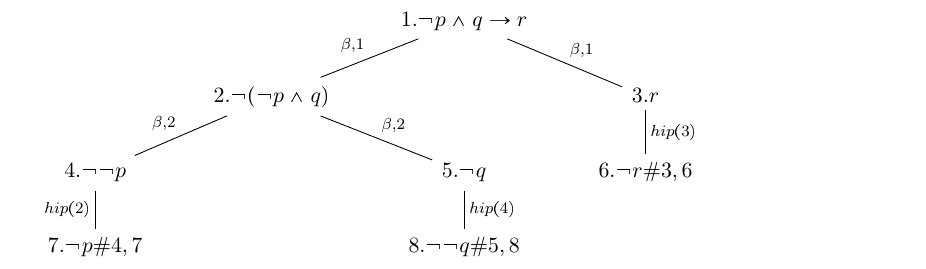
\includegraphics[scale = 0.63]{figures/tableau1.png}
\end{center}


Recordemos que el \textit{tableau} se construye de arriba hacia abajo. Por la regla $R_{ini}$, el grafo de un solo vértice $\neg p \land q \to r$ es un \textit{tableau} de $\Psi$, ya que $\neg p \land q \to r \in\Psi$. $\\$
Ahora  bien, $\neg p \land q \to r$ es una $\beta$-fórmula de tipo $\beta=\varphi_1\to\varphi_2$, de modo que, atendiendo a la tabla de las $\beta$-fórmulas, se descompone en las fórmulas $\beta_1=\neg\varphi_1=\neg(\neg p\land q)$ y $\beta_2=\varphi_2=r$.$\\$
Teniendo la descomposición de la $\beta$-fórmula, podemos aplicar la regla $R_\beta$, y obtenemos un \textit{tableau} con dos ramificaciones, una con $\neg(\neg p\land q)$ y otra con $r$:
\begin{itemize}
    \item Comenzamos con la segunda rama, que es la más sencilla. Usando la regla $R_{hip}$, podemos añadir a la rama cualquier elemento de $\Psi$, de modo que escogemos $\neg r$. Ahora bien, en esta rama tenemos las proposiciones $\neg p \land q \to r$, $r$ y $\neg r$. En concreto, tenemos las proposiciones $r$ y $\neg r$. Como en la rama hay dos proposiciones de tipo $\varphi$ y $\neg \varphi$, es cerrada y hemos acabado con ella. Simbolizaremos que una rama está cerrada escribieno $\#$ y señalando los vértices en los que se encuentran las proposiciones contradictorias.
    \item Fijémonos ahora la rama de $\neg(\neg p\land q)$. De nuevo, tenemos una $\beta$-fórmula. Usando la tabla como  antes, vemos que se descompone en $\beta_1=\neg\neg p$, $\beta_2=\neg q$. De modo que, por la regla $R_\beta$, esta rama se divide a su vez en otras dos:
    \begin{itemize}
        \item La primera rama tiene los elementos $\neg p \land q \to r$, $\neg(\neg p\land q)$ y $\neg\neg p$. Usando la regla $R_{hip}$, podemos añadir a esta rama el elemento $\neg p$ de $\Psi$. Ahora, dos de los elementos de esta rama son $\neg\neg p$ y $\neg p$. Es decir, tenemos las fórmulas $\varphi$ y $\neg\varphi$, siendo $\varphi=\neg p$. Por tanto esta rama está cerrada.
        \item La segunda rama tiene los elementos $\neg p \land q \to r$, $\neg(\neg p\land q)$ y $\neg q$. Usando la regla $R_{hip}$, podemos añadir a esta rama el elemento $\neg\neg q$ de $\Psi$. Ahora, dos de los elementos de esta rama son $\neg\neg q$ y $\neg q$. Como la rama contiene una fórmula y su negación, es cerrada.
    \end{itemize}
    
\end{itemize}

Como todas las ramas son cerradas, el \textit{tableau} es cerrado.$\\$
\end{example}

Vemos a continuación otro ejemplo en el que no se cumple que $\Phi\vDash\varphi$. Es decir, hay una valoración que cumple $\Phi$ y $\neg\varphi$. En estos casos, veremos que no se puede conseguir un \textit{tableau} cerrado de $\Phi\cup\{\neg\varphi\}$. Al intentar obtener un \textit{tableau} cerrado, la complicación del método aumentará considerablemente pero también nos dará indicaciones sobre qué valoración de verdad satisface a $\Phi$ y $\neg\varphi$.
\begin{example}
Sea $\varphi=\neg(p_3\to p_6)$ y $\Phi$ formado por estas seis proposiciones:
\begin{enumerate}
    \item $p_1\to(p_2\lor p_3)$
    \item $\neg p_1\to(p_3\lor p_4)$
    \item $p_1\to\neg p_6$
    \item $\neg p_3\to (p_4\to p_1)$
    \item $\neg(p_2\land p_5)$
    \item $p_2\to p_5$
\end{enumerate}
Intentemos conseguir un \textit{tableau} cerrado de $\Phi\cup\{\neg\varphi\}$:

% https://tikzcd.yichuanshen.de/#N4Igdg9gJgpgziAXAbVABwnAlgFyxMJZABgBoBGAXVJADcBDAGwFcYkQ0B9AZgAIAdfgCcsAcwAWOekKEQA7ry4A2EAF9S6TLnyEUZAEzU6TVu0FgYoxTzUaOWvASLlShmgxZtEHTivWbsR11kF24jD1NvLnIBYTFJaVkFc0trPzsMQJ1nUgAWcJMvEBSrZVsA7ScUfTyCzzN+C1LOcnL7LKrkGoBWOsiQWKbrGMERCSkZeV4ACi4+QUYIIWtcgEo2zMrgmqU+opKS4Y2HbJRuUl33QvY52MXlrlzjjuDzgHY9hqHb0fiJpJmj1iYwSkwU0XW-naWyI5wAHJ8opxcsC-okptFnjCULlSAirvVvIdDnMsUEiLiAJyInwjOLjdEKWacfR3JbWbiQjInTq48jEGlcVkLdmkqGbckoboUAUE-oklpk07IaXkKhy-aNVLM4X8Rj0MBQazdLkVSUqihuYyE4pa5rdJWdJSWmkK-SO4LO8hhDU3Fmohlg40eohe-K+pEO8U84JvCjh63yu3Wd3Rl5EOPkXoRnzcEN6UiyxOapolZnzemggHKSFGGBQUTwIigABmsgAtkgyCAcBAkC4QOIYPQoOxIBYQDR9QAjGCMAAKMfYIJwk+LDVnUjabYgncQNR7fcQ3Znc8X6e8K7XEU1m-o247SHOh6QB5v7HEWDQD93T5ovaQXFB2HUdvHHNgp3oWcFyXS8-mva4iX4O8fz3aUX0QZ9Txgi8QCvHNBBQqEdz3Z0MPQ99vE-b9iMfRA4X-I8yOw89sTw+CCOQmAt1o39EDIgDEDjYCRzHAgIJAFjYPY8YEJtQjuPvXi90pRikAY9cqK-VD+wHQTVMkqCz2k-DNNtIi7BIpADME-kaCHUSwPEuSkxQyDoNYyUZMkHTEHIA9bIHSjB205T+wCo9vXskCxInTi3MMjyTPgsK-KA2y30Q8zFLXKTcKvVKszUtL3OM3DGBgFtVxzajfKKjDyDIhzQPAZz4py0qcLYgrLLo8hhNsiisoUrdOs805vNXQqNNs4Tgtq1L9G7WyNOCkb7zG5LZOm4ryAM5rYokvLuo4sz1t8-Q9KPJbOOwUR2yU3q+OW67Mvk-g7oetRKFUIA
% https://tikzcd.yichuanshen.de/#N4Igdg9gJgpgziAXAbVABwnAlgFyxMJZABgBpiBdUkANwEMAbAVxiRAB12wYBzT7ngAo0AfQDMAAk4AnLDwAWOOtOkQA7hNEA2AJQgAvqXSZc+QijIBGKrUYs2oyTLmLlqjdoNGQGbHgJEZABMNvTMrIgcXLya4l7GfmZElqQh1GH2kZ6GCaYBKClioXYRPiKWUuyyCkoq6pUCsVrxPib+5sgpACzF4Wz8MdnevnkdQaQ96SX90Tyxli0j7UTjAKy9mVGNohXONW71wuKVDBDSsV16Oa2J+cjjWhulA3yz84ttSShipI9TfVljpxTudRF0PrcOj8AOxPGbbIFVFy1dwSI5dSrVVx1DzlK7DT53H4ADjhgIxe2xqJ2ENGRC6pFJ-02Lwagzi1yWX2QDIAnGSyrskfscWjREETmdYmJ8blligGZZKMzSuLJaCOQTIURVqQlQLWTTOYSOrrLNYVfCYkcJcC6GAoLFVrKbnSUGa0rYAVt2atafLkFo9Z6Ms83uL-dyg5YipbAbbhVT6qI-cbtSho5MvZsU5G7tC9VnQ1a5hG027kAXLOs42UxAYbDAoDx4ERQAAzVQAWyQKRAOAgSHG2dKACURJwAEYwJQgagMOjThgABRNbCxODnIHkMDoUDYkG4LU7EB7iD7A6QZBHbHHnGwPC7dC3C6Xq-TIAYMHbm+oO73SBgEwDAMNcJ5nj8-aDuetZ3uw06zvOi4wCua6RBux7dkgDJQUgkHFpE47APIWBoPoL7IahH5fj+mGnth1CXoguo3oRE7wTOz5IW+aEgBhf67vukSHqwYFYYgQa4YgOEESAcEIVxn6Ue+bp8cidFngWUmSbJREkWRFE8dR36bmJ9GIFpTHErB7EKYZKEqfKak1Fu-5CeABCid44FILyjHQVpum2Zx9lUapGFmWeSr+b5NnEaR5HcQ5vE0aZ3nidFUnmjZU4hUlYVOfx26CQenkab2w5MZlQW5YhSlGeF6mRb2kFVcOQXxQZ+WOV8n4meV56tdBlgydMbG1Ypr7JR+RVuaVR7NeeLFVfhY1ycFdVTQVvURel5mWJJVUsR1+mJfV02qalA0HTF56BWt8l5ed235M5iiuSVwllYtljWVlOkPRtk3Kbxu0dhlflZX9J0JaFPWvVdP2Q0xQTXjVHGbSDM3qQJAFfQte1nkEF7DZD6N2d1oNNYTQ6VdBxM5ewD5PnDKX9foFD6EAA
\begin{comment}
\begin{center}
\begin{tikzcd}
\neg\neg(p_3 \rightarrow p_6)                                            &                                                                              &                                                                                         &                                                                                                &                                                                                    &                                                                          &                                                                         &                                 \\
p_3 \rightarrow p_6 \arrow[d, "R_\beta"', no head] \arrow[u, "R_\sigma"] &                                                                              &                                                                                         &                                                                                                &                                                                                    &                                                                          &                                                                         &                                 \\
\neg p_3                                                                 & p_6 \arrow[lu, "R_\beta"']                                                   &                                                                                         &                                                                                                &                                                                                    &                                                                          &                                                                         &                                 \\
                                                                         & p_1 \rightarrow \neg p_6 \arrow[u, "R_{hip}"] \arrow[d, "R_\beta"', no head] &                                                                                         &                                                                                                &                                                                                    &                                                                          &                                                                         &                                 \\
                                                                         & \neg p_6                                                                     & \neg p_1 \arrow[lu, "R_\beta"']                                                         &                                                                                                &                                                                                    &                                                                          &                                                                         &                                 \\
                                                                         &                                                                              & \neg p_1 \rightarrow (p_3 \lor p_4) \arrow[u, "R_{hip}"] \arrow[d, "R_\beta"', no head] &                                                                                                &                                                                                    &                                                                          &                                                                         &                                 \\
                                                                         &                                                                              & \neg\neg p_1                                                                            & p_3 \lor p_4 \arrow[lu, "R_\beta"']                                                            &                                                                                    &                                                                          &                                                                         &                                 \\
                                                                         &                                                                              &                                                                                         & \neg p_3 \rightarrow (p_4 \rightarrow p_1) \arrow[u, "R_{hip}"] \arrow[d, "R_\beta"', no head] &                                                                                    &                                                                          &                                                                         &                                 \\
                                                                         &                                                                              &                                                                                         & p_4 \rightarrow p_1                                                                            & \neg \neg p_3 \arrow[lu, "R_\beta"']                                               &                                                                          &                                                                         &                                 \\
                                                                         &                                                                              &                                                                                         &                                                                                                & p_1 \rightarrow (p_2 \lor p_3) \arrow[u, "R_{hip}"] \arrow[d, "R_\beta"', no head] &                                                                          &                                                                         &                                 \\
                                                                         &                                                                              &                                                                                         &                                                                                                & p_2 \lor p_3                                                                       & \neg p_1 \arrow[lu, "R_\beta"']                                          &                                                                         &                                 \\
                                                                         &                                                                              &                                                                                         &                                                                                                &                                                                                    & \neg (p_2 \land p_5) \arrow[u, "R_{hip}"] \arrow[d, "R_\beta"', no head] &                                                                         &                                 \\
                                                                         &                                                                              &                                                                                         &                                                                                                &                                                                                    & \neg p_5                                                                 & \neg p_2 \arrow[lu, "R_\beta"']                                         &                                 \\
                                                                         &                                                                              &                                                                                         &                                                                                                &                                                                                    &                                                                          & p_2 \rightarrow p_5 \arrow[u, "R_{hip}"] \arrow[d, "R_\beta"', no head] &                                 \\
                                                                         &                                                                              &                                                                                         &                                                                                                &                                                                                    &                                                                          & p_5                                                                     & \neg p_2 \arrow[lu, "R_\beta"'] \\
                                                                         &                                                                              &                                                                                         &                                                                                                &                                                                                    &                                                                          &                                                                         & p_3 \arrow[u, "R_\sigma"]      
\end{tikzcd}
%Otra versión (la otra no cabe)
\begin{tikzcd}
1.\neg\neg(p_3 \rightarrow p_6)                                   &                                                           \\
2.p_3 \rightarrow p_6 \arrow[u, "{\sigma,1}"]                     &                                                           \\
4.p_6 \arrow[u, "{\beta,2}"]                                      & 3.\neg p_3 \arrow[lu, "{\beta,2}"', no head]              \\
5.p_1 \rightarrow \neg p_6 \arrow[u, "hip(3)"]                    &                                                           \\
7.\neg p_1 \arrow[u, "{\beta,5}"]                                 & {6.\neg p_6\#4,6} \arrow[lu, "{\beta,5}"', no head]       \\
8.\neg p_1 \rightarrow (p_3 \lor p_4) \arrow[u, "hip(2)"]         &                                                           \\
10.p_3 \lor p_4 \arrow[u, "{\beta,8}"]                            & {9.\neg\neg p_1\#7,9} \arrow[lu, "{\beta,8}"', no head]   \\
11.\neg p_3 \rightarrow (p_4 \rightarrow p_1) \arrow[u, "hip(4)"] &                                                           \\
13.\neg \neg p_3 \arrow[u, "{\beta,11}"]                          & 12.p_4 \rightarrow p_1 \arrow[lu, "{\beta,11}"', no head] \\
14.p_1 \rightarrow (p_2 \lor p_3) \arrow[u, "hip(1)"]             &                                                           \\
16.\neg p_1 \arrow[u, "{\beta,14}"]                               & 15.p_2 \lor p_3 \arrow[lu, "{\beta,14}"', no head]        \\
17.\neg (p_2 \land p_5) \arrow[u, "hip(5)"]                       &                                                           \\
19.\neg p_2 \arrow[u, "{\beta,17}"]                               & 18.\neg p_5 \arrow[lu, "{\beta,17}"', no head]            \\
20.p_2 \rightarrow p_5 \arrow[u, "hip(6)"]                        &                                                           \\
22.\neg p_2 \arrow[u, "{\beta,20}"]                               & 21.p_5 \arrow[lu, "{\beta,20}"', no head]                 \\
23.p_3 \arrow[u, "{\sigma,13}"]                                   &                                                          
\end{tikzcd}
\end{center}
\end{comment}

\begin{figure}[H]
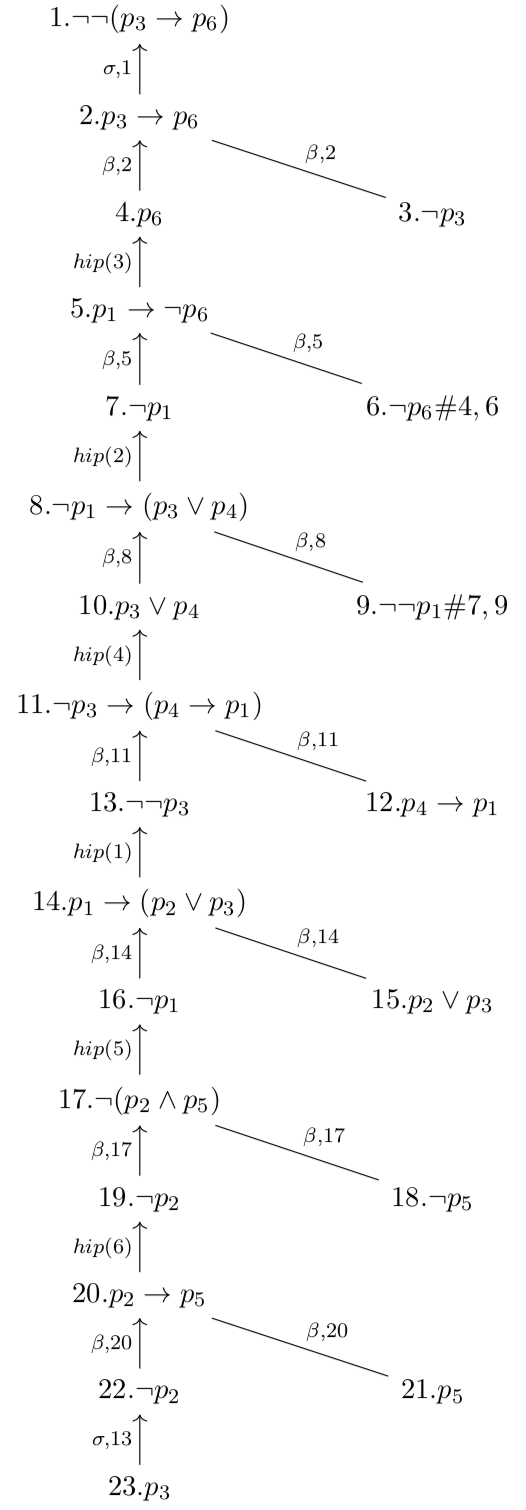
\includegraphics[scale = 0.57]{figures/tableau2.png}
\end{figure}

Como podemos ver, no conseguimos cerrar las ramas. En la rama que hemos indicado con flechas, no parece haber forma de encontrar una contradicción, y además tenemos en esta rama las proposiciones $\neg p_1$, $\neg p_2$, $p_3$ y $p_6$. En este caso podemos imaginar que la rama no se puede cerrar y hay una valoración que cumple los elementos de esa rama. En efecto, solo tenemos 4 opciones en función de los valores de verdad que asociemos a $p_4$ y $p_5$, y encontramos que la valoración dada por $v(p_1)=v(p_2)=v(p_5)=F$,$v(p_3)=v(p_4)=v(p_6)=V$ cumple $\Phi$ y $\neg\varphi$. Es decir, $\Phi\nvDash\varphi$. Como veremos en breve, esto significa que no podemos encontrar un  tableau cerrado para $\Phi\cup\{\neg\varphi\}$.

\end{example}



Ahora bien, nuestro objetivo inicial era, dados un conjunto de fórmulas $\Phi$ y una fórmula $\varphi$, demostrar usando el método de los \textit{tableaux} que $\Phi\vDash\varphi$. Por tanto, para que el método nos permita alcanzar este objetivo tiene que cumplir dos propiedades:
\begin{itemize}
    \item \textit{Completitud:} $\Phi \vDash \varphi$ implica $\Phi \vdash_{tb} \varphi$.
    Es decir, si se cumple que $\Phi\vDash\varphi$, entonces podemos encontrar un \textit{tableau} cerrado para $\Phi\cup\{\neg\varphi\}$.
    \item \textit{Corrección:} $\Phi \vdash_{tb} \varphi$ implica $\Phi \vDash \varphi$.
    Es decir, si encontramos un \textit{tableau} cerrado para $\Phi\cup\{\neg\varphi\}$, entonces se cumple que $\Phi\vDash\varphi$. 
\end{itemize}